\subsection{Process pinning}

%%%%%%%%%%%%%%%%%%%%%%%%%%%%%%%%%%%%%%%%%%%%%%%%%%%%%%%%%%
\begin{frame}[t]{Explicit MPI Process Pinnning}
\small
\justifying
To make process pinning \textbf{deterministic}, a python script was developed to automatically generate \textbf{rankfiles} based on the number of \textbf{MPI processes}, \textbf{OpenMP threads} per MPI process, the maximum number of processing elements and the number of \textbf{NUMA domains}.


\begin{figure}
	\centering
	\begin{tabular}{cc}
		\subfloat[Spread]{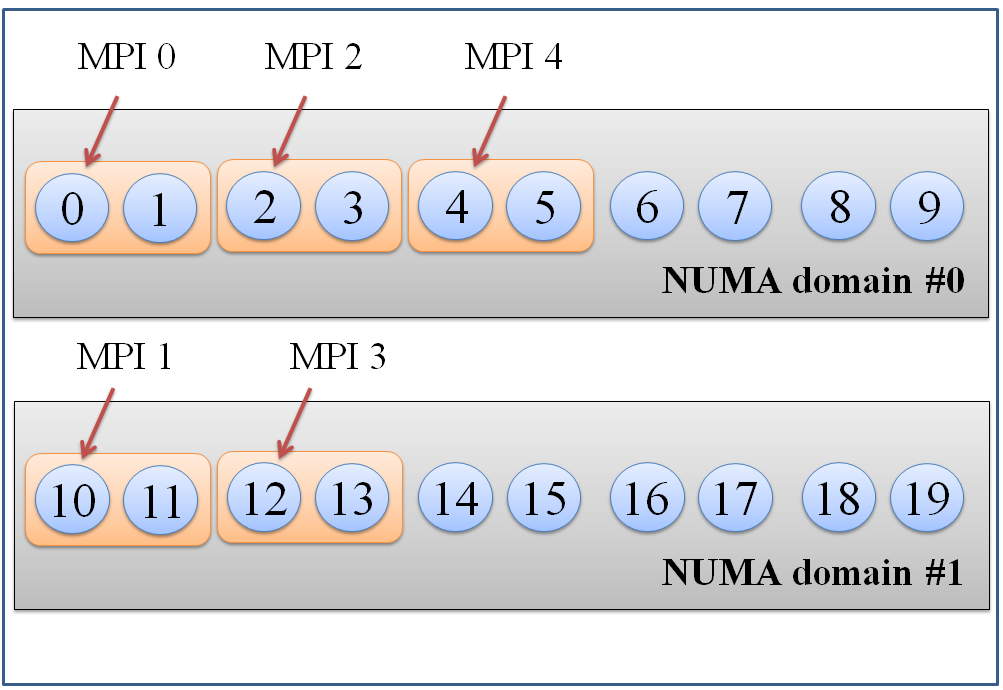
\includegraphics[width=0.4\textwidth]{figures/chapter-2/spread-mode.png} \label{fig:mm-parallel-model-tree-linear}} & 
		\subfloat[Close]{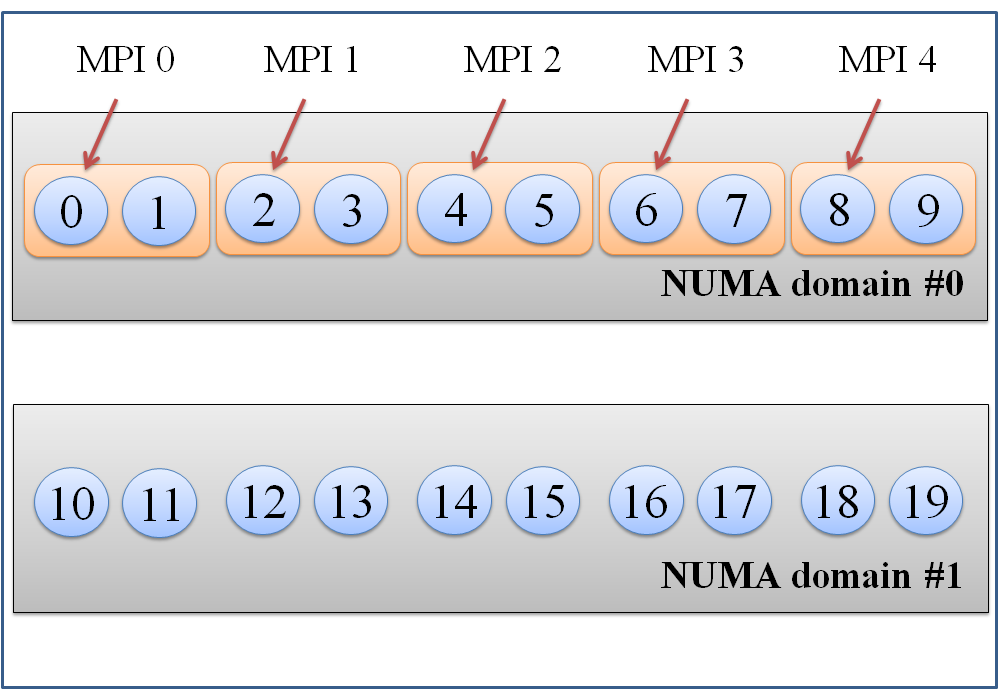
\includegraphics[width=0.4\textwidth]{figures/chapter-2/close-mode.png} \label{fig:mm-parallel-model-tree-quadratic}} \\
	\end{tabular}
	\caption{Process pinning of 2 OpenMP / 1 MPI on HW1 hardware}
	\label{fig:python-script-rankfile-example}
\end{figure}

\end{frame}